\documentclass[a4paper, 12pt]{article}

\usepackage[english,russian]{babel}
\usepackage[T2A]{fontenc}
\usepackage[utf8]{inputenc}
\usepackage{geometry}
\usepackage{enumitem}
\usepackage{setspace}
\usepackage{amssymb}
\usepackage{graphicx}
\usepackage{wrapfig}
\usepackage{float}
\usepackage{amsmath}
\usepackage{textcomp}
\usepackage{dsfont}

\geometry{top=5mm, left=1cm}
%\setlength{\parindent}{0}
\renewcommand{\arraystretch}{1.2}
\linespread{1}

\begin{document}
    \begin{center}
        \textbf{Сферическая геометрия №4}\\
        Фигуры.
    \end{center}


    \textbf{№ 1}
    Пусть $n$ - число углов в фигуре, какое минимальное $n$ возможно на евклидовой плоскости?
    А на сферической?
    Дайте ее определение, найдите площадь такой сферической фигуры, если для нее известны все углы.

    \begin{center}
        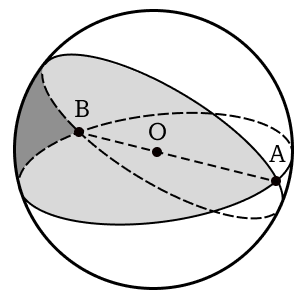
\includegraphics[width=0.2\textwidth]{images/Frame 52}\\
    \end{center}
    \textbf{Решение}\\
    На евклидовой плоскости такая фигура треугольник,
    двуугольник невозможен, так как он является вырожденным треугольником, то есть прямой.\\

    На сфере такая фигура - двуугольник - фигура, ограниченная двумя прямыми.\\

    Найдем площадь двуугольника.\\
    Заметим, что двуугольник с углом $\alpha$ занимает $\frac{\alpha}{2\pi}$ часть всей сферы,
    тогда так как площадь всей сферы равна $4\pi R^2$, то площадь двуугольника равна
    \[
        \frac{\alpha}{2\pi}\cdot 4\pi R^2 = 2\alpha R^2\text{ где $\alpha$ в радианах}
    \]\\


    \textbf{№ 2}
    Дайте определение сферического треугольника, его сторон, углов, вершин.
    Найдите его площадь.

    \textbf{Решение}\\
    \begin{center}
        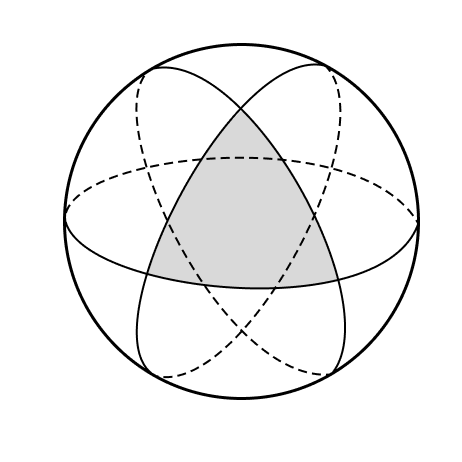
\includegraphics[width=0.2\textwidth]{images/Frame 23}\\
    \end{center}

    1) Три большие окружности на сфере, не пересекающиеся в одной
    точке, делят сферу на восемь областей.
    Каждая из этих областей, ограниченная дугами трех больших
    окружностей, называется сферическим треугольником.
    Дуги больших окружностей, ограничивающие сферический треугольник, называются
    его сторонами, концы этих дуг называются его вершинами, а углы, образуемые сторонами сферического треугольника в его вершинах, называются углами сферического треугольника.

    2) Площадь:
    \begin{center}
        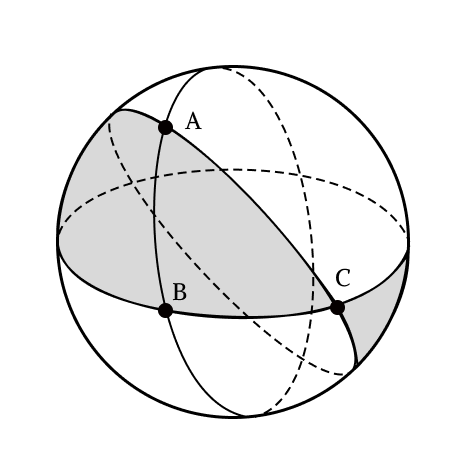
\includegraphics[width=0.2\textwidth]{images/Frame 24}\\
    \end{center}

    У треугольника 3 угла, и 3 угла вертикальные с ними.
    Эти 6 углов образуют 6 двуугольников, которые в сумме содержат площади 6 искомых треугольников
    (3 спереди сферы и 3 сзади).
    Кроме того, они покрывают всю сферу, то есть сумма площадей всех двуугольников равна

    \[
        2S_A + 2S_B + 2S_C = S_{\text{сферы}} + 4S_{\triangle ABC}
    \]

    Распишем площади двуугольников и сферы:
    \[
        2 \cdot \frac{A}{2\pi}\cdot 4\pi R^2 + 2 \cdot \frac{B}{2\pi}\cdot 4\pi R^2 + 2 \cdot \frac{B}{2\pi}\cdot 4\pi R^2 =
        4\pi R^2 + 4S_{\triangle ABC}
    \]
    \[
        4R^2(A + B + C) = 4\pi R^2 + 4S_{\triangle ABC}
    \]
    \[
        4S_{\triangle ABC} = 4R^2(A + B + C) - 4\pi R^2
    \]
    \[
        S_{\triangle ABC} = R^2(A + B + C - \pi)
    \]\\


    \textbf{№ 3}
    Сравните сумму углов треугольника на сфере и на евклидовой плоскости.
    Выведите формулу, вычисляющую сферический «дефект».
    Возможен ли треугольник, у которого все углы $90^\circ$,
    а треугольник все стороны которого лежат на экваторе?
    Найдите их стороны и площади.

    \textbf{Решение}\\

    1) Из формулы площади следует, что сумма углов сферического треугольника всегда больше $\pi$,
    то насколько она больше $\pi$ называется сферическим дефектом:
    \[
        \delta = A + B + C - \pi
    \]
    \begin{center}
        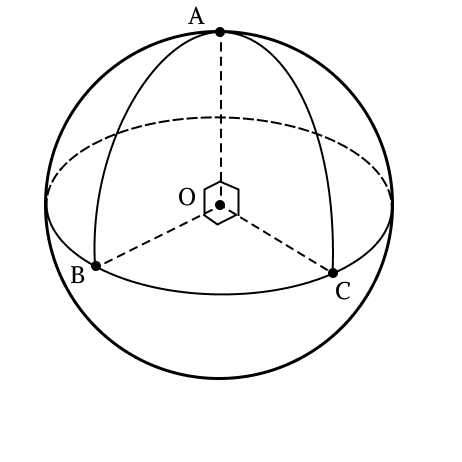
\includegraphics[width=0.2\textwidth]{images/img6}\\
    \end{center}

    2) Треугольник с попарно перпендикулярными сторонами:
    такой треугольник образуют три попарно перпендикулярные сферические прямые.

    \[
        \cup AB = \cup AC = \cup BC = \frac{\pi}{2}R
    \]
    \[
        S = R^2\left(\frac{3\pi}{2} - \pi\right) = R^2 * \frac{\pi}{2}
    \]

    Ответ: стороны равны:$\frac{\pi}{2}R$; площадь: $R^2 * \frac{\pi}{2}$

    3) Треугольника с тремя вершинами на экваторе не существует.\\
    Рассмотрим прямую, являющуюся экватором и две другие прямые, пересекающие ее.
    Одна прямая пересекается по точкам диаметрально противоположным и другая прямая также
    пересекает по диаметрально противоположным точкам, то есть две не экваториальные прямые
    не могут пересекаться на экваторе, так как тогда из этой точки пересечения можно провести два диаметра.\\


    \textbf{№ 4}
    Выведите формулу для площади сферического $n$-угольника и формулу сферического дефекта для него.

    \textbf{Решение}\\

    Полная индукция $S = R^2\left(\displaystyle\sum_{i=1}^n A_i\right) - \pi(n - 2)$:\\

    \textbf{1)База}: треугольник, двуугольник.\\

    \textbf{2) Переход}:
    Разобьем $n$ - угольник на $n - 2$ треугольника,
    тогда по предположению индукции и свойству площади целой фигуры по частям имеем:
    \[
        S_n = \displaystyle\sum_{i=1}^{n-2} S_i = R^2\left(\displaystyle\sum_{i=1}^n A_i\right) - \pi(n - 2)
    \]

    Дефект вычисляется следующим образом:
    \[
        \left(\displaystyle\sum_{i=1}^n A_i\right) - \pi(n - 2)
    \]\\


    \textbf{№ 5}
    На сфере дан треугольник $\triangle ABC$, на уго сторонах $AB$ и $AC$ взяли
    точки $P$ и $Q$ так, что $\angle APQ = \angle ABC$ и $\angle AQP = \angle ACB$.
    Найдите площадь $PQCB$.
    \begin{center}
        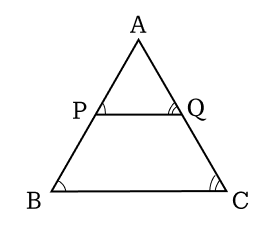
\includegraphics[width=0.2\textwidth]{images/Frame 72@2x}\\
    \end{center}

    Посчитаем сумму всех углов четырехугольника:
    \[
        \angle B + \angle APQ + \angle CQP + \angle C =
        \angle B + \pi - \angle APQ + \pi - \angle PQA + \angle C =
        \angle B + \pi - \angle B + \pi - \angle C + \angle C = 2\pi
    \]
    Посчитаем площадь:
    \[
        S = 2\pi - 2\pi = 0
    \]

    Это означает, что треугольники совпадают и на сфере нет подобных треугольников.\\


    \textbf{№ 6}
    Проверьте, всегда ли медианы сферического треугольника пересекаются в одной точке?
    А высоты и биссектрисы?

    \begin{center}
        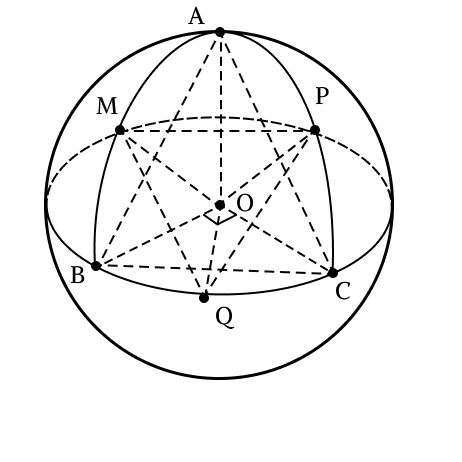
\includegraphics[width=0.2\textwidth]{images/Frame 73}\\
    \end{center}

    1) Медианы.\\

    Проведем много треугольников.
    Понятно, что $OM$, $OP$, $OQ$ лежат в одной плоскости с сферическими медианами.
    $AB || PQ$, значит плоскость проходит по медиане в треугольнике $MQP$ из точки $M$.
    Для других точке аналогично.
    Получаем, что «медианные плоскости» пересекаются по прямой O-точка пересечения медиан MPQ,
    а значит сферические прямые пересекаются по точке.\\

    2) Про биссектрисы аналогично.

    \begin{center}
        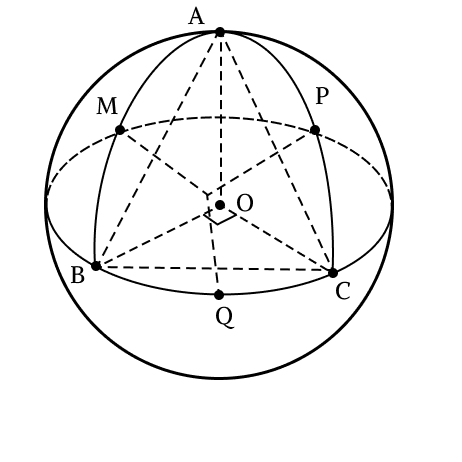
\includegraphics[width=0.2\textwidth]{images/Frame 74}\\
    \end{center}

    3) Для высот рассматриваем перпендикулярные плоскости.\\


    \textbf{№ 7}
    Когда для сферического треугольника существует описанная окружность?

    \textbf{Решение}\\

    Через вершины треугольника можно провести плоскость, она задает окружность на сфере,
    значит для любого сферического треугольника можно построить описанную окружность.\\


    \textbf{№ 10}
    Чему равна площадь сферического треугольника, образованного полюсом и двумя сопряженными с ним точками,
    если сферическое расстояние между этими точками равно $h$, а радиус сферы равен $R$.

    \textbf{Решение}\\

    \begin{center}
        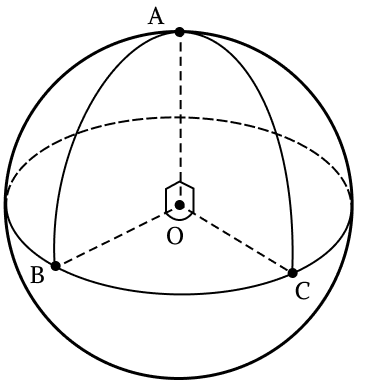
\includegraphics[width=0.2\textwidth]{images/img5}\\
    \end{center}

    1)
    \[
        \angle B = \angle C = \frac{\pi}{2}
    \]
    \[
        \angle A = \frac{h}{R}
    \]

    2) \[
           S_{\triangle ABC} = R^2(\angle A + \angle B + \angle C - \pi) = R^2\frac{h}{R}
    \]

    Ответ: $R^2\frac{h}{R}$\\


    \textbf{№ 11}
    Дан сферический треугольник с площадью $S$.
    Найдите площадь треугольника с такими же углами на сфере с вдвое большим радиусом.

    \textbf{Решение}\\

    \[
        S_1 = R^2(\angle A + \angle B + \angle C - \pi)
    \]
    \[
        S_2 = (2R)^2(\angle A + \angle B + \angle C - \pi) = 4R^2(\angle A + \angle B + \angle C - \pi) = 4S_1
    \]

    Ответ: $4S$\\


    \textbf{№ 12}
    Два диаметра, соединяющих пары полюсов пересекаются под углом $\alpha$,
    чему равны площади двуугольников, образованных их полярами, если радиус сферы равен $R$?

    \textbf{Решение}\\

    1) Как было доказано на занятии 2 в номере 7, угол между диаметрами, соединяющими полюсы,
    равен углу между полярами этих полюсов, тогда на сфере получится два вида двуугольников,
    площадь которых равны:

    \[
        S_1 = 2\alpha \cdot R
    \]
    \[
        S_2 = 2(\pi - \alpha) \cdot R
    \]\\

    Ответ: $2\alpha \cdot R $; $2(\pi - \alpha) \cdot $\\


    \textbf{№ 13}
    На сфере даны два равнобедренных треугольника, имеющих один равный угол.
    Отношение углов при основании первого треугольника ко второму равно $\delta$.
    Найдите отношение площадей этих треугольников

    \textbf{Решение}\\

    1)
    \[
        S_2 = R ^ 2(A + 2B - \pi)
    \]
    \[
        S_1 = R^2(A + 2B\delta - \pi)
    \]
    2)
    \[
        \frac{S_1}{S_2} = \frac{R ^ 2(A + 2B - \pi)}{R ^ 2(A + 2B\delta - \pi)} = \frac{(A + 2B - \pi)}{(A + 2B\delta - \pi)}
    \]

    Ответ: $\frac{(A + 2B - \pi)}{(A + 2B\delta - \pi)}$\\


    \textbf{№ 14}
    На сфере дан треугольник, все углы которого равны $90^\circ$.
    На одну из сторон опустили медиану.
    Найдите чему равна площадь получившихся треугольников, если площадь изначального треугольника равна $S$.

    \textbf{Решение}\\

    \begin{center}
        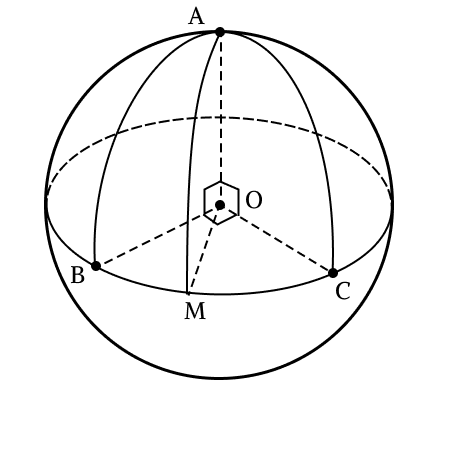
\includegraphics[width=0.2\textwidth]{images/img9}\\
    \end{center}

    1) $AO\bot BOC$ по признаку перпендикулярности прямой и плоскости, тогда $(MOA)\bot(BOC)$ по признаку перпендикулярности
    плоскостей.
    Получаем, что в сферическом треугольнике $\triangle ABM$ $\angle B = \angle M = 90^\circ$

    2) Осталось найти $\angle A$.
    Он равен линейному углу $\angle BOM$
    Так как $\cup BM = \cup MC$, то $\angle BOM \angle MOC = 45^\circ = \frac{\pi}{4}$

    3) Таким образом, искомая площадь равна:
    \[
        S = R^2(\angle BAM + \angle AMB + \angle MBA - \pi) =
        R^2\left(\frac{\pi}{4} + \frac{\pi}{2}+ \frac{\pi}{2} - \pi\right) =
        \frac{R^2\pi}{4}
    \]
    Площадь начального треугольника равна:
    \[
        S_0 = \frac{R^2\pi}{2} \rightarrow S = \frac{S_0}{2}
    \]

    Ответ:$\frac{S_0}{2}$

\end{document}
